\documentclass{standalone}
\usepackage{tikz}
\usepackage{circuitikz}

\begin{document}
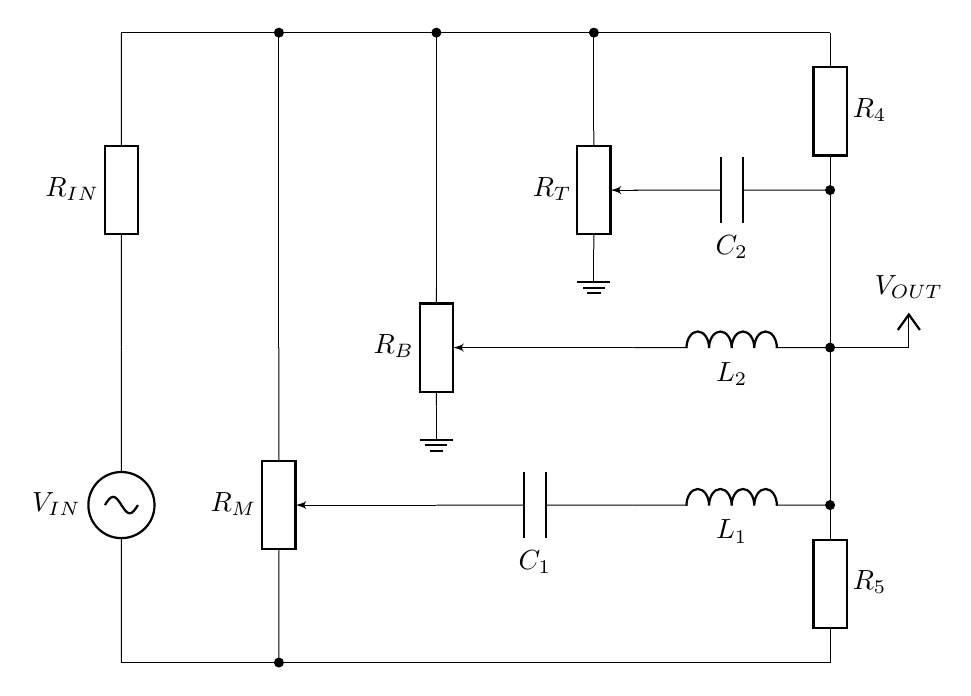
\begin{tikzpicture}
	\draw (1, 5) to[sinusoidal voltage source, l_=$V_{IN}$] (1, 1);

	\draw (1, 5) to[european resistor, l=$R_{IN}$] (1, 9);
	\draw (10, 7) to[european resistor, l_=$R_4$] (10, 9);
	\draw (10, 3) to[european resistor, l=$R_5$] (10, 1);

	\draw (5, 5.75) to[european potentiometer, l_=$R_B$] (5, 4.25);
	\draw (3, 5) to[european potentiometer, l_=$R_M$] (3, 1);
	\draw (7, 7.75) to[european potentiometer, l_=$R_T$] (7, 6.25);

	\draw (7.5, 3) to[capacitor, l=$C_1$] (5, 3);
	\draw (10, 7) to[capacitor, l=$C_2$] (7.5, 7);

	\draw (7.5, 3) to[american inductor, l_=$L_1$] (10, 3);
	\draw (7.5, 5) to[american inductor, l_=$L_2$] (10, 5);

	\draw (10, 1) -- (1, 1);
	\draw (1, 9) -- (10, 9);
	\draw (3, 5) -- (3, 9);
	\draw (3.56, 3) -- (5, 3);
	\draw (5, 5.75) -- (5, 9);
	\draw (5.56, 5) -- (7.5, 5);
	\draw (7, 7.75) -- (7, 9);
	\draw (10, 7) -- (10, 3);
	\draw (10, 5) -- (11, 5);

	\node[ground] at (5, 4.25) {};
	\node[ground] at (7, 6.25) {};
	\node[vcc] at (11, 5) {$V_{OUT}$};
	\node[circ] at (10, 3) {};
	\node[circ] at (10, 5) {};
	\node[circ] at (10, 7) {};
	\node[circ] at (3, 1) {};
	\node[circ] at (3, 9) {};
	\node[circ] at (5, 9) {};
	\node[circ] at (7, 9) {};

\end{tikzpicture}
\end{document}